\documentclass[times]{elsarticle}


\usepackage[dvipsnames]{xcolor}
\usepackage{amsmath}
\usepackage{amsfonts}
\usepackage{amssymb}
\usepackage{lineno}
\usepackage{enumerate}
\usepackage{times}
\usepackage{subcaption}
\usepackage{graphicx,psfrag}
\usepackage[skip=0pt]{caption}


\newcommand\solidrule[1][0.25cm]{\rule[0.5ex]{#1}{1pt}}
\newcommand\dashedrule{\mbox{%
  \solidrule[2mm]\hspace{2mm}\solidrule[2mm]}}

\newcommand{\dotrule}[1]{%
	\parbox{#1}{\dotfill}} 

\makeatletter
\newcommand \Dotfill {\leavevmode \cleaders \hb@xt@ .22em{\hss .\hss }\hfill \kern \z@}
\makeatother
 
\newcommand{\Dotrule}[1]{%
   \parbox{#1}{\Dotfill}} 

\begin{document}

\title{Behaviour of the Serre Equations in the Presence of Steep Gradients Revisited}

\author[ANU]{J.P.A.~Pitt\corref{cor1}}
\ead{jordan.pitt@anu.edu.au }
\author[ANU]{C.~Zoppou}
\ead{christopher.zoppou@anu.edu.au}
\author[ANU]{S.G.~Roberts}
\ead{stephen.roberts@anu.edu.au}

\cortext[cor1]{Corresponding author}
\address[ANU]{Mathematical Sciences Institute, Australian National University, Canberra, ACT 0200, Australia}
 \begin{abstract}

 \end{abstract}	
 
  \begin{keyword}
  	Serre equations\sep steep gradients \sep dam break
  \end{keyword}
  
 \maketitle
\linenumbers
%--------------------------------------------------------------------------------
\section{Introduction} \label{intro} 

\section{Serre Equations}
\label{section:Serre Equations}
The Serre equations can be derived by integrating the full incompressible Euler equations over the water depth, see for example \cite{Su-Gardener-1969-536}. They can also be derived as an asymptotic expansion of the Euler equations, see for example \cite{Bonneton-Lannes-2009-16601}. Assuming a constant horizontal bed the one-dimensional Serre equations are \cite{Guyenne-etal-2014-169}
\begin{linenomath*}
\begin{subequations}\label{eq:Serre_nonconservative_form}
\begin{gather}
\dfrac{\partial h}{\partial t} + \dfrac{\partial (uh)}{\partial x} = 0
\label{eq:Serre_continuity}
\end{gather}
and
\begin{gather}
\underbrace{\underbrace{\dfrac{\partial (uh)}{\partial t} + \dfrac{\partial}{\partial x} \left ( u^2h + \dfrac{gh^2}{2}\right )}_{\text{Shallow Water Wave Equations}} + \underbrace{\dfrac{\partial}{\partial x} \left (  \dfrac{h^3}{3} \left [ \dfrac{\partial u }{\partial x} \dfrac{\partial u}{\partial x} - u\dfrac{\partial^2 u}{\partial x^2}  - \dfrac{\partial^2 u}{\partial x \partial t}\right ] \right )}_{\text{Dispersion Terms}} = 0.}_{\text{Serre Equations}}
\label{eq:Serre_momentum}
\end{gather}
\end{subequations}
\end{linenomath*}
Where $u$ is the  horizontal velocity over the depth of water $h$, $g$ is the acceleration due to gravity, $x$ is the horizontal spatial variable and $t$ is time. 

\subsection{Conservation Laws}
The Serre equations are derived from conservation laws for mass ($h$) and momentum ($uh$) \cite{Su-Gardener-1969-536} thus our numerical methods should conserve these quantities. The total amount of a quantity $q$ in a system ocurring on the interval $[a,b]$ is measured by
\begin{linenomath*}
\begin{gather*}
\label{eqn:Condef}
\mathcal{C}_q(t) = \int_{a}^{b} q(x,t)\, dx .
\end{gather*}
\end{linenomath*}
Conservation of a quantity $q$ implies that $\mathcal{C}_{q}(0) = \mathcal{C}_{q}(t)$ $\forall t$ provided the interval is fixed and the system is closed. Our methods should have this property for the quantities $h$ and $uh$. Additionally the Serre equations admit a Hamiltonian \cite{Li-Y-2002,Green-Naghdi-1976-237}
\begin{linenomath*}
\begin{gather}
\label{eqn:Hamildef}
\mathcal{H}(x,t) = \frac{1}{2} \left(hu^2 + \frac{h^3}{3} \left(\frac{\partial u}{\partial x}\right)^2 + gh^2\right)
\end{gather}
\end{linenomath*}
which should also be conserved. The Hamiltonian is the sum of the kinetic energies in the horizontal ($hu^2$) and vertical (${h^3} \left({\partial u}/{\partial x}\right)^2 /{3}$) directions and the gravitational potential energy ($gh^2$).  

\section{Numerical Methods}
%where methods come from
%grid and cells definition
In Section \ref{section:NumRes} five different numerical methods are used the first ($\mathcal{V}_1$), second ($\mathcal{V}_2$) and third-order ($\mathcal{V}_3$) methods of \cite{Zoppou-etal-2017}, the method of \citet{El-etal-2006} ($\mathcal{E}$) and a second-order finite difference method ($\mathcal{G}$). These methods all use a fixed grid in time and space, with subscripts denoting spatial indices and superscripts denoting time indices. Thus for a quantity $q$ on our grid $q_i^n = q(x_i,t^n)$ with the grids uniform such that $\Delta x = x_{i} - x_{i-1}$ $\forall i$ and $\Delta t = t^{n} - t^{n-1}$ $\forall n$. A cell is a particularly useful unit of the finite volume method, the $i$th cell is the interval [$x_i -\Delta x/2$,$x_i +\Delta x/2$] centered around $x_{i}$.

All methods are stable under the CFL condition \cite{Harten-etal-1983-357}. For completness the two methods $\mathcal{G}$ and $\mathcal{E}$ which are not explicitly published are presented in the Appendix to allow for replication.

%--------------------------------------------------------------------------------
\section{Smoothed Dam Break Problem}
\label{section:smootheddambreak}
%--------------------------------------------------------------------------------
%put background in here more on the rerasion for doing this smoothing

The discontinuous dam-break problem can be approximated smoothly using the hyperbolic tangent function. Such an approximation will be called a smoothed dam-break problem and will be defined as such
\begin{linenomath*}
\begin{subequations}
\begin{gather}
h(x,0) = h_0 + \frac{h_1 - h_0}{2}\left(1 + \tanh\left(\frac{x_0 - x}{\alpha}\right)\right),
\end{gather}
\begin{gather}
u(x,0) = 0.0m/s.
\end{gather}
\label{eq:sdbi}
\end{subequations}
\end{linenomath*}
Where $\alpha$ measures the distance over which $46.117\%$ of the smooth transition between the two heights of $h_0$ and $h_1$ centered around $x_0$ occurs. Figure \ref{fig:dbsmoothinit} demonstrates the effect of varying $\alpha$ for the smoothed dam-break problem with $h_1 =1.8m$, $h_0 = 1m$ and $x_0 = 500m$. These are the same $h_0$ and $h_1$ values as those of the dam-breaks presented by \cite{El-etal-2006} and \cite{Hank-etal-2010-2034} and will be the values used in Sections \ref{section:smootheddambreak} and \ref{section:NumRes}.
\begin{figure}
\centering
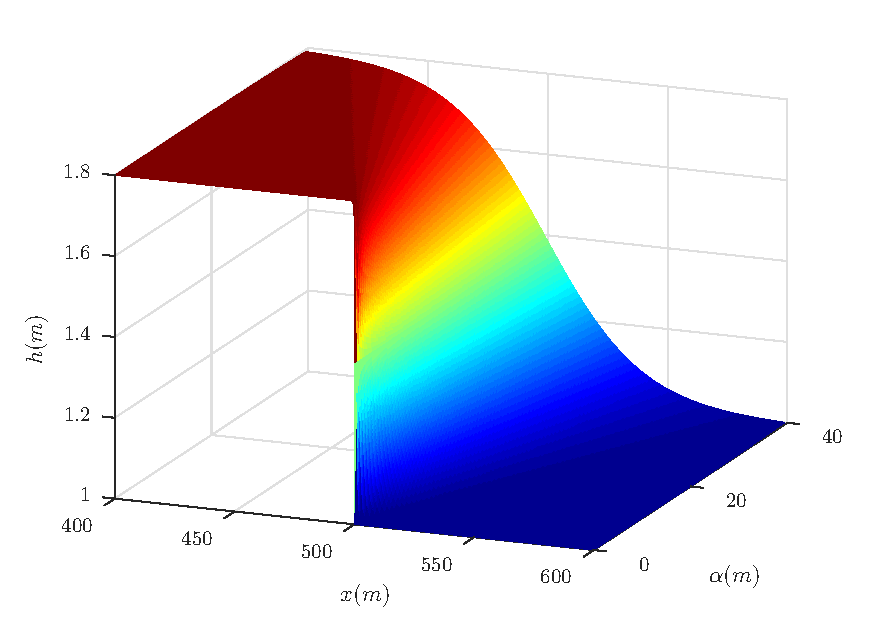
\includegraphics[width=0.6\textwidth]{pics/explainers/dbs.pdf}
\caption{Initial conditions for the smooth dam-break problem with $h_0 = 1m$, $h_1 = 1.8m$ and $x_0 =500m$ as $\alpha$ varies.}
\label{fig:dbsmoothinit}
\end{figure}
%
\subsection{Measures and Comparisons}
%Intro
There are no analytic results for the Serre equations for either the discontinous dam-break problem or its smoothed approximant. To assess the validity of our results we must resort to other comparisons such as measuring the error in the conservation of the conserved quantities and measuring the distance between numerical solutions as $\Delta x \rightarrow 0$. \citet{Hank-etal-2010-2034} and \citet{Mitsotakis-etal-2014} demonstrated that the analytic solution of the shallow water wave equations for the dam-break problem captures the mean behaviour of their numerical results. While \citet{El-etal-2006} derived expressions for the leading wave height and speed of an undular bore in the Serre equations. We make use of all of these comparions in Section \ref{section:NumRes} and so we present some relevant background for each here. 

%define cells%

\subsubsection{Conserved Quantities}
The initial conditions of the smoothed dam-break \eqref{eq:sdbi} were integrated to get the following expressions for $C_{h}(0)$, $C_{uh}(0)$ and $C_{\mathcal{H}}(0)$ provided $x_0$ is the midpoint of the spatial domain $\left[a,b \right]$ in which the smoothed dam-break occurs
\begin{linenomath*}
	\begin{subequations}
	\begin{gather*}
	\mathcal{C}_{h}(0) = \frac{h_1 + h_0}{2}\left(b- a\right),
	\label{eq:Chdef}
	\end{gather*}
	\begin{gather*}
	\mathcal{C}_{uh}(0) = 0
	\label{eq:Cuhdef}
	\end{gather*}
		and
	\begin{gather*}
	\mathcal{C}_{\mathcal{H}}(0) = \frac{g}{4} \left(h_0^2 - h_1^2 + \alpha\left(h_1 - h_0\right)^2\tanh\left(\frac{a - b}{2 \alpha}\right)\right).
	\label{eq:CHdef}
	\end{gather*}
		\label{eq:Canalyticvalues}	
	\end{subequations}
\end{linenomath*}

To calculate the total amount of a quantity $q$ in our numerical solution we fit a quartic interpolant of the primitive variables $h$ and $u$ over a cell utilising neighbouring cells and then apply Gaussian quadrature with 3 points to get the total amount of $q$ in a cell and then sum this for all cells to get the total amount of $q$ in our numerical solution at time $t$ which we call $\mathcal{C^*}_{q}(t)$. We then measure the error in conservation of a quantity $q$ for a numerical method by
\begin{linenomath*}
		\begin{gather}
		C_1^q = \frac{\left| \mathcal{C}_{q}(0) - \mathcal{C^*}_{q}(t) \right| }{\left|\mathcal{C}_{q}(0)\right|}.
		\end{gather}
\end{linenomath*}
Note that for $uh$ the denominator is $0$ and that there is a flux of momentum due to the unequal heights at both ends of the domain. To resolve these issues for $uh$ we measure the error in the conservation by
\begin{linenomath*}
	\begin{gather}
	C_1^{uh} = \left| \mathcal{C}_{q}(0) - \mathcal{C^*}_{q}(t) - \frac{gt}{2}\left(h(b)^2 - h(a)^2\right)\right|  .
	\label{eq:C1def}
	\end{gather}
\end{linenomath*}
\subsubsection{Distance between Numerical Results}
By measuing the relative distance between results we can assess whether our numerical solutions are converging as $\Delta x  \rightarrow 0$. Rather than comparing all numerical results to one another we simplify by comparing all our numerical solutions to the one with the smallest $\Delta x$. For some quantity $q$ we have a numerical approximation to it $q'$ at the locations $x_i$ and our numerical approximation to it with smallest $\Delta x$ $q^*$ at the locations $x_j$. By using grids such that for each $i$ there is a $j^*(i)$ such that $x_i = x_{j^*(i)}$ by summing the difference for each $i$
\begin{linenomath*}
	\begin{gather}
	L_1^{q} = \dfrac{\sum_{i} \left| q'_i  - q^*_{j^*(i)}\right|}{\sum_{i} \left| q^*_{j^*(i)}\right|}
	\label{eq:L1def}
	\end{gather}
\end{linenomath*}
we can measure the relative distance between these numerical solutions on the grid $x_i$.

\subsubsection{Shallow Water Wave Equation Analytic Solution for the Dam Break}
For the discontinous dam break problem the shallow water wave equations which are the Serre equations with dispersive terms neglected can be solved analytically. The analytic solution of the shallow water wave equations have been used as a comparative tool against numerical results in the literature \cite{Hank-etal-2010-2034,Mitsotakis-etal-2014} as they appear to capture the mean behaviour of the numerical solutions. 

An example of the analytic solution of the shallow water wave equations for the dam-break problem is presented in Figure \ref{fig:SWWEanadiagram} at $t=30s$. Region I is the undisturbed water upstream of the dam-break at constant height ($h_1$) and velocity ($0m/s$) and region II is the rarefaction fan connecting regions I and III. Regions III and IV are the constant height ($h_2$) and constant velocity ($u_2$) state which are seperated by $x_{u_2} = x_0 + u_2t$ and region V is the undisturbed water downstream at constant height ($h_0$) and velocity ($0m/s$) seperated from region IV by a shock which travels at velocity $S_2$. Expressions for the unknown quantities $h_2$, $u_2$ and $S_2$ in terms of $h_0$ and $h_1$ were given by \citet{Wu-etal-1999-1210}
\begin{linenomath*}
\begin{subequations}
\begin{gather}
h_2 = \frac{h_0}{2} \left(\sqrt{1 + 8 \left(\frac{2h_2}{h_2 - h_0}\frac{\sqrt{gh_1} - \sqrt{gh_2}}{\sqrt{gh_0}}\right)^2} - 1\right),
\end{gather}
	\begin{gather}
	u_2 = 2\left(\sqrt{gh_1} - \sqrt{gh_2}\right)
	\end{gather}
and
	\begin{gather}
	S_2 = \frac{h_2 u_2}{h_2 - h_0}.
	\end{gather}
\label{eq:WuSWWE}	
\end{subequations}
\end{linenomath*}
From these values the location of the shock seperating regions IV and V at time $t$ is $x_{S_2}(t) = x_0 + S_2t$. Applying \eqref{eq:WuSWWE} to our dam-break problem heights then $h_2 = 1.36898m$ , $u_2 = 1.074975$ $m/s$ and $S_2 = 3.98835$ $m/s$ which are demonstrated in Figure \ref{fig:SWWEanadiagram}.


\subsubsection{Whitham Modulation for Undular Bores of the Serre Equations}
Undular bores for the one dimensional Serre equations were analysed by \cite{El-etal-2006} and an expression for the amplitude ($A^+$) and speed ($S^+$) of the leading wave of a bore shown in Figure \ref{fig:Serreanadiagram} were given
\begin{linenomath*}
	\begin{subequations}
\begin{gather}
\frac{\Delta}{\left(A^+ + 1\right)^{1/4}} - \left(\frac{3}{4 -  \sqrt{A^+ + 1}}\right)^{21/10} \left(\frac{2}{1 + \sqrt{A^+ + 1}}\right)^{2/5} = 0
\label{eq:aplusdef}
\end{gather}
and
\begin{gather}
S^+ = \sqrt{g \left(A^+ + 1\right)}
\label{eq:splusdef}
\end{gather}
		\label{eq:ELWhitMod}	
	\end{subequations}
\end{linenomath*}
where $\Delta = h_b / h_0$, and $h_b$ is the amplitude of the bore. From this we define $x_{S^+}(t) = x_0 + S^+t$ which is the location of the leading wave at time $t$.
For \eqref{eq:ELWhitMod} the height of the bore created by the dam-break is \cite{El-etal-2006}
\begin{gather*}
\label{eqn:hrdef}
h_b = \frac{1}{4}\left(\sqrt{\frac{h_1}{h_0}} + 1\right)^2.
\end{gather*} 
Thus for our dam-break problem heights $h_b = 1.37082$ $m$, $\Delta = 1.37082$,  $A^+ = 1.73998$ $m$ and $S^+ = 4.13148$ $m/s$.

\begin{figure}
\centering
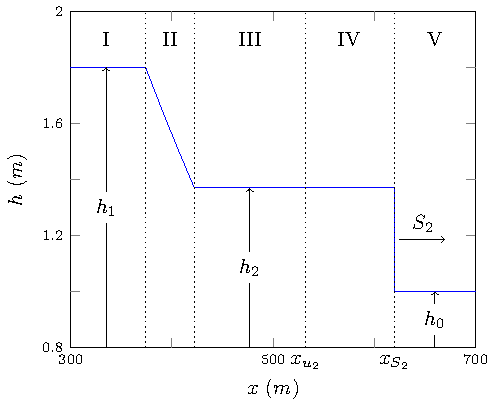
\includegraphics[width=0.5\textwidth]{pics/explainers/SWWEana.pdf}
\caption{Analytic solution at $t=30s$ of the shallow water wave equations for the dam-break problem with $h_0 = 1m$, $h_1=1.8m$ and $x_0=100m$.}
\label{fig:SWWEanadiagram}
\end{figure}

\begin{figure}
\centering
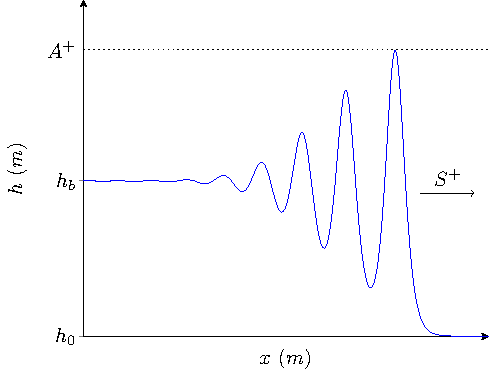
\includegraphics[width=0.5\textwidth]{pics/explainers/SERREex.pdf}
\caption{Demonstration of quantities obtained by Whitham modulation for undular bores of the Serre equations.}
\label{fig:Serreanadiagram}
\end{figure}



%--------------------------------------------------------------------------------
\section{Numerical Results}
\label{section:NumRes}
%--------------------------------------------------------------------------------
%Intro
We begin by looking into the effect of the initial steepness of the smoothed dam-break problem for different $\alpha$ values by observing what happens as $\Delta x \rightarrow 0$ and our numerical solutions better approximate the true solution of the Serre equations. To have the smallest error we use the highest order well validated model $\mathcal{V}_3$ in the following investigation. From these results we then investigate numerical results for long time scales, how the shallow water wave equations analytic solution and El's Whitham modulation values compare to our results and then finally present some other findings about the behaviour of our numerical solutions. 

All numerical methods used $\Delta t = 0.01 \Delta x$ which is much smaller than required by the CFL condition \cite{Harten-etal-1983-357} which ensures stability of our schemes or the relation used by \cite{El-etal-2006}. $\Delta t$ was chosen to be much smaller than necessary because for a final time of $t=30s$ making $\Delta t$ small suppresses errors without excessivly increasing the runtime of the experiments. $\mathcal{V}_2$ requires an input parameter to its slope limiter and this was chosen to be $\theta = 1.2$ \cite{Zoppou-etal-2017}. 

\subsection{Effect of $alpha$}
We observe that there are four types of behaviour as $\Delta x \rightarrow 0$ depending on the $\alpha$ and the numerical method. The four behaviours are identified by the nature of the solutions around $x_{u_2}$ when $\Delta x$ is small and they correspond to different results presented in the literature. For brevity the only given examples of these behaviours will be the solutions of $\mathcal{V}_3$ at $t=30s$ on the interval $x\in[0m,1000m]$ although they all also occurred for the numerical results of $\mathcal{E}$, $\mathcal{G}$ and $\mathcal{V}_2$ using the same $\alpha$ and $\Delta x = 10/2^{10}m$. All of the numerical methods presented use dirichlet boundary conditions with $u = 0m/s$ at both boundaries and $h =1.8m$ on the left and $h =1m$ on the right.

\subsubsection{Non-oscillatory Behaviour}
The first behaviour which will be referred to as the non-oscillatory behaviour has such smooth initial conditions that no oscillations were introduced by $t= 30s$ for the numerical simulations, although given sufficient time the front steepens and an undular bore will develop. This behaviour is not present in the literature as no authors chose large enough $\alpha$. An example of this behaviour can be seen in Figure \ref{fig:o3a1dxlimflatexp} for $\alpha = 40m$ using $\mathcal{V}_3$ this behaviour was also observed for $\mathcal{V}_1$'s numerical solutions. Because this is a very smooth problem we observe that all numerical results are visually identical for all $\Delta x < 10 / 2^4m$. We note that $\mathcal{V}_3$'s numerical solution has $h(x_{u_2}) > h_2$ and because no undulations are present the results of \citet{El-etal-2006} are not applicable to these solutions.   

From Table \ref{tab:L1C1} it can be seen that the numerical solutions of $\mathcal{V}_3$ conserve the conserved quantities very well for this particular $\alpha$ for both $\Delta x$'s, although the smaller $\Delta x$'s numerical results are superior. $C^{uh}_1$ is the worst performing of the measures because the smoothed dam-break has such a large transition width that $h(0m) \neq 1.8m$ and $h(1000m) \neq 1m$ causing small unquantifiable flows at the boundaries meaning the system is not closed. 

These measures verify that we are converging as $\Delta x \rightarrow 0$ and our solutions are relatively conservative as the errors for the highest resolution results except for $C^{uh}_1$ are all at round-off error for each cells value as there are $100,000$ cells. Therefore the numerical result in Figure \ref{fig:o3a1dxlimflatexp} is an accurate representation of the behaviour of the Serre equations when $\alpha$ is sufficiently large and in particular $\alpha = 40m$. 
\begin{table}
	\centering
	{\renewcommand{\arraystretch}{1.2}
		\begin{tabular}{c c  c  c  c c  c }
			$\alpha$ ($m$)&$\Delta x$ ($m$)& $C^h_1$  & $C^{uh}_1$ & $C^\mathcal{H}_1$ & $L^h_1$  & $L^{u}_1$  \\
			\hline \hline
			$40$ &	${10}/{2^{4}}$ & $2.0\times 10^{-11}$ &  $1.8 \times 10^{-6}$ & $1.2 \times 10^{-8}$ &  $1.7 \times 10^{-7}$ & $2.9 \times 10^{-6}$ \\
			$40$ &	${10}/{2^{10}}$ & $1.8\times 10^{-11}$ &  $2.2 \times 10^{-8}$ & $3.6 \times 10^{-11}$ &  $2.5\times 10^{-11}$ & $6.5\times 10^{-11}$ \\
			\hline
			$2$ &	${10}/{2^{4}}$ & $4.9\times 10^{-14}$ &  $5.1\times 10^{-3}$ & $8.7 \times 10^{-4}$  & $5.0\times 10^{-3}$ & $6.8\times 10^{-2}$ \\
			$2$ &	${10}/{2^{10}}$ & $4.0\times 10^{-12}$ &  $5.0 \times 10^{-9}$ & $2.0 \times 10^{-8}$ &  $1.8\times 10^{-7}$ & $2.3\times 10^{-6}$  \\
			\hline
			$0.4$ &	${10}/{2^{4}}$ & $9\times 10^{-14}$ &  $4.8\times 10^{-3}$ & $1.0 \times 10^{-3}$ & $6.8\times 10^{-3}$ $\dagger$ & $9.9\times 10^{-2}$ $\dagger$\\
			$0.4$ &	${10}/{2^{10}}$ & $3.9\times 10^{-12}$ &  $5.0 \times 10^{-9}$ & $2.0 \times 10^{-8}$  &   $3.6\times 10^{-7}$ $\dagger$ &  $5.0\times 10^{-6}$ $\dagger$\\
			\hline
			$0.1$ &	${10}/{2^{4}}$ & $7.6\times 10^{-14}$ &  $4.8\times 10^{-3}$ & $1.0 \times 10^{-3}$ &  $7.0\times 10^{-3}$ $\dagger$ &   $1.0\times 10^{-1}$ $\dagger$ \\
			$0.1$ &	${10}/{2^{10}}$ & $3.9\times 10^{-12}$ &  $4.6 \times 10^{-8}$ & $7.6 \times 10^{-7}$  & $5.0\times 10^{-7}$ $\dagger$ & $6.4\times 10^{-6}$ $\dagger$  \\
			\hline \hline
		\end{tabular}
		}
		\caption{All errors in conservation $C^{q}_1$ \eqref{eq:C1def} for the conserved quantities and relative distances $L^{q}_1$ \eqref{eq:L1def} of the primitive variables for numerical solutions of $\mathcal{V}_3$. $L^{q}_1$ uses the numerical solution with $\Delta x = 10/2^{11}m$ as the high resolution basis of comparison and $\dagger$ indicates where the interval [$520m$, $540m$] has been omitted from the comparison.}
		\label{tab:L1C1}
\end{table}


\begin{figure}
\centering
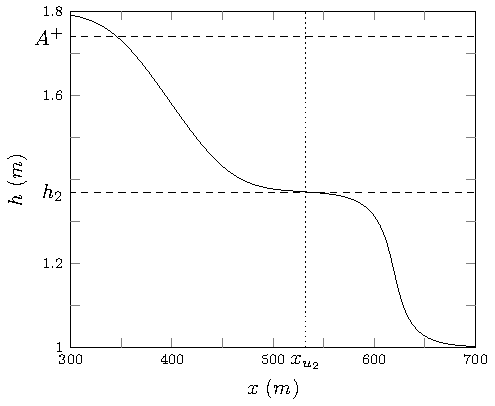
\includegraphics[width=0.7\textwidth]{pics/results/SDB/numsols/alpha0.025/1-figure0.pdf}
\caption{Numerical results of $\mathcal{V}_3$  at $t= 30s$ for the smooth dam-break problem with $\alpha = 40m$ for $\Delta x = 10/2^{4}m$ ({\color{black} \solidrule}).}
\label{fig:o3a1dxlimflatexp}
\end{figure}
%

\subsubsection{Flat Behaviour}
The second behaviour will be referred to as the flat behaviour due to the presence of a constant height around $x_{u_2}$, this is the most common behaviour observed in the literature \cite{Hank-etal-2010-2034,Mitsotakis-etal-2014,Mitsotakis-etal-2017}. This behaviour has oscillations in regions III and IV which are seperated by a constant height state around $x_{u_2}$. An example of the numerical results for this behaviour can be seen in Figure \ref{fig:o3a6dxlimflatexp} when $\alpha = 2m$, this behaviour was also observed for $\mathcal{V}_1$'s solutions.

As $\Delta x$ decreases the numerical solutions converge so that by $\Delta x = 10 / 2^8m$ the solutions for higher $\Delta x$ are visually identical. There is also good agreement between the peak amplitude in region IV ($A$) and $A^+$ as well as $h(x_{u_2})$ and $h_2$. Although as $\Delta x$ is decreased in the simulations we observe $h(x_{u_2}) > h_2$. Since this method is well validated for smooth problems and a small $\Delta x$ has been chosen this suggests that the mean bore heights in regions III and IV from a dam-break may differ slightly between the shallow water wave equations and the Serre equations. These solutions replicate the behaviour of the results of \citet{Mitsotakis-etal-2017} who use the same $\alpha$ but different $h_0$ and $h_1$.

Table \ref{tab:L1C1} demonstrates good conservation of the conserved quantities for our numerical solution with $\Delta x = 10 / 2^{10}m$, although only the errors in conservation of $h$ are at the size of round-off errors. The $L_1$ measures demonstrate that our solutions are very close to the numerical solution with $\Delta x = 10 / 2^{11}m$. 

These results demonstrate that the numerical solutions in Figure \ref{fig:o3a6dxlimflatexp} are an accurate representation of the nature of the Serre equations provided $\alpha$ and $\Delta x$ are appropriate supporting the numerical solutions of \cite{Mitsotakis-etal-2017} who used the same $\alpha$ but different $h_0$ and $h_1$ values.

\begin{figure}
\centering
\begin{subfigure}{\textwidth}
	\centering
	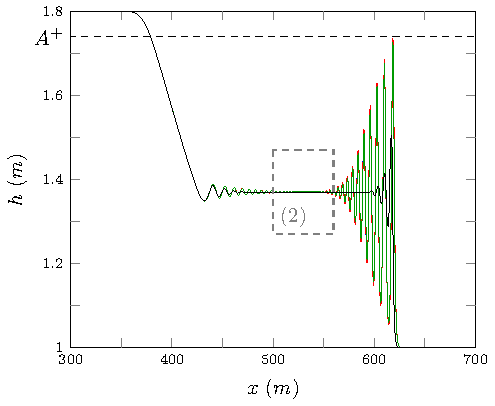
\includegraphics[width=0.7\textwidth]{pics/results/SDB/numsols/alpha0.5/1-figure0.pdf}
\end{subfigure}
\begin{subfigure}{\textwidth}
	\centering
	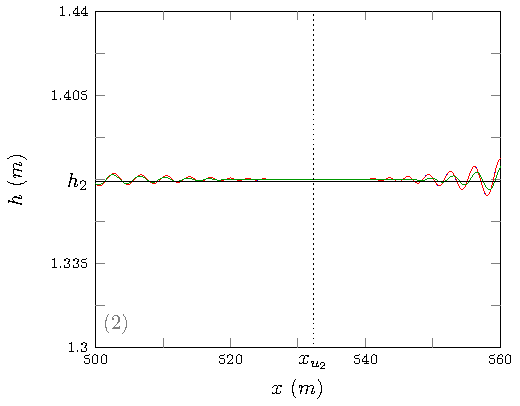
\includegraphics[width=0.5\textwidth]{pics/results/SDB/numsols/alpha0.5/2-figure0.pdf}
\end{subfigure}
\caption{Numerical results of $\mathcal{V}_3$  at $t= 30s$ for the smooth dam-break problem with $\alpha = 2m$ for $\Delta x = 10/2^{10}m$ ({\color{blue} \solidrule}), $10/2^8m$ ({\color{red} \solidrule}), $10/2^6m$ ({\color{green!60!black} \solidrule}) and $10/2^{4}m$ ({\color{black} \solidrule}).}
\label{fig:o3a6dxlimflatexp}
\end{figure}


\subsubsection{Node Behaviour}
The third behaviour will be referred to as the node behaviour and it is was observed by \cite{El-etal-2006}. The node behaviour's main feature is that the oscillations in region III and IV decay and appear to meet at $x_{u_2}$ as can be seen in Figure \ref{fig:o3a9dxlimcdexp} when $\alpha = 0.4m$. Unfortunatly these numerical solutions are not visually identical for the higher resolutions as they were in the flat behaviour example. However, the numerical solutions are getting closer to one another and convergence is expected for the smaller $\Delta x$ because the problem is still smooth. In these results $A^+$ is a good estimator for $A$ and the oscillations in regions III and IV appear to be around $h_2$. This behaviour was observed by \cite{El-etal-2006} for $\mathcal{E}$ and indeed we have replicated it. This behaviour was not observed in $\mathcal{V}_1$'s solutions up to $\Delta x=10/2^{10}m$ with $\alpha=0.001m$ as $\mathcal{V}_1$ introduces diffusive errors that severly dampen oscillations. This explains why \cite{Hank-etal-2010-2034} using $\mathcal{V}_1$ could not replicate the results of \cite{El-etal-2006}. It was found that an $\alpha$ of at least $0.4m$ is required to recover the node behaviour this explains why \citet{Mitsotakis-etal-2014} and \citet{Mitsotakis-etal-2017} using $\alpha$'s of $2m$ and $1m$ respectively could not replicate the results of \citet{El-etal-2006}. 

Figure \ref{fig:o3a9dxlimcdexp} demonstrates that our numerical solutions have not converged, however this is only in the area around $x_{u_2}$. This indicates that the behaviour of our solutions away from $x_{u_2}$ are consistent, in particular our results for $A$. The larger distance between numerical solutions means we cannot get a meaningful measure of $L_1$ for the whole domain. However, by omitting an interval around $x_{u_2}$ such as [$520m$, $540m$] a meaningul measure of $L_1$ can be calculated, this modified $L_1$ is presentedd in Table \ref{tab:L1C1}. These modified $L_1$'s demonstrate that our solutions are close to one another and have converged away from $x_{u_2}$, so that increasing the grid resolution further would only cause a significant change in the numerical solutions around $x_{u_2}$. Table \ref{tab:L1C1} shows that for $\Delta x = 10/2^{10}m$ our conserved quantities are very well conserved by our numerical solution.

These results suggest that although we have not yet fully converged these numerical solutions are close to reasonable solutions of the Serre equations for the smoothed dam-break problem for an appropriate $\alpha$ value supporting the numerical solutions presented by \citet{El-etal-2006}.
\begin{figure}
\centering
\begin{subfigure}{\textwidth}
	\centering
	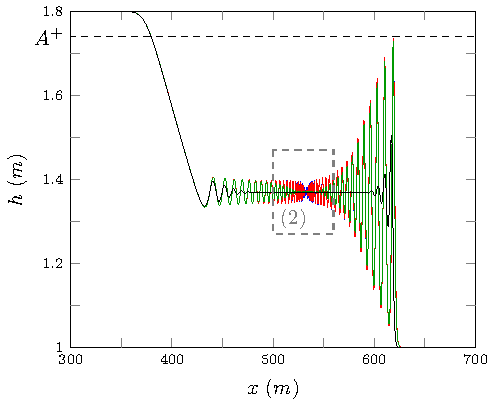
\includegraphics[width=0.7\textwidth]{pics/results/SDB/numsols/alpha2.5/1-figure0.pdf}
\end{subfigure}
\begin{subfigure}{\textwidth}
	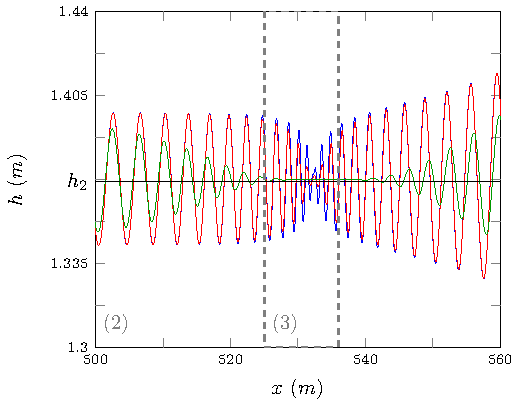
\includegraphics[width=0.5\textwidth]{pics/results/SDB/numsols/alpha2.5/2-figure0.pdf}
	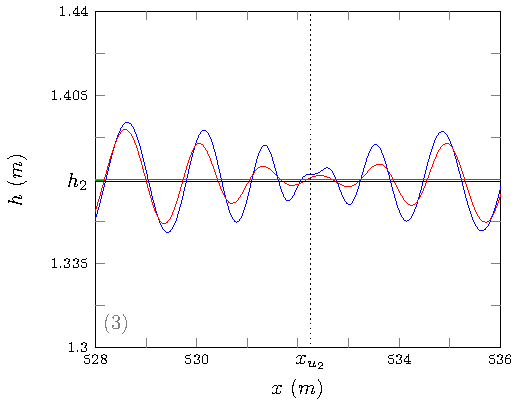
\includegraphics[width=0.5\textwidth]{pics/results/SDB/numsols/alpha2.5/3-figure0.pdf}
\end{subfigure}
\caption{Numerical results of $\mathcal{V}_3$  at $t= 30s$ for the smooth dam-break problem with $\alpha = 0.4m$ for $\Delta x = 10/2^{10}m$ ({\color{blue} \solidrule}), $10/2^8m$ ({\color{red} \solidrule}), $10/2^6m$ ({\color{green!60!black} \solidrule}) and $10/2^{4}m$ ({\color{black} \solidrule}).}
\label{fig:o3a9dxlimcdexp}
\end{figure}


\subsubsection{Growth Behaviour}
The fourth behaviour will be referred to as the growth behaviour due to the oscillations in regions III and IV growing around $x_{u_2}$ as can be seen in Figure \ref{fig:o3a20dxlimcdexp} for $\alpha = 0.1m$. This behaviour could not be replicated for $\mathcal{V}_1$ and has hitherto not been published. 

Figure \ref{fig:o3a20dxlimcdexp} shows that the disagreement in the numerical results is concentrated around $x_{u_2}$. $A$ is again predicted by $A^+$ well and the oscillations in regions III and IV are around $h_2$. The different resolution numerical results are getting closer to one another, but the sudden change in behaviour around $x_{u_2}$ makes it difficult to assert that large growths in amplitude are not possible around $x_{u_2}$ as we take $\Delta x$ smaller. However, for numerical solutions with $\alpha = 0.001m$ and $\Delta x = 10 / 2^{11}m$ these oscillations around $x_{u_2}$ stayed within the interval [$1.455m$,$1.3m$]. The number of oscillations is the same for $\Delta x = 10 / 2^{10}m$ in Figures \ref{fig:o3a9dxlimcdexp} and \ref{fig:o3a20dxlimcdexp} with different $\alpha$ values so that the change in behaviour is a result of the difference in amplitudes of the oscillations and not an increase in their number.

The interval [$520m$,$540m$] has been omitted from $L_1$ in Table \ref{tab:L1C1} due to the lack of convergence in this region. The $L_1$ measures for the numerical solution with $\alpha = 0.1m$ and $\Delta x = 10/2^{10}m$ are very close but slightly larger than those for the node behaviour, confirming that our numerical solutions are correctly capturing the behaviour of the Serre equations for this problem away from $x_{u_2}$. The errors in conservation are small, and in particular our conservation of $h$ is as good as those in node and flat behaviour. The errors in conservation of $uh$ and $\mathcal{H}$ however are larger than the previous behaviours examples by a factor of $10$.


\begin{figure}
\centering
\begin{subfigure}{\textwidth}
	\centering
	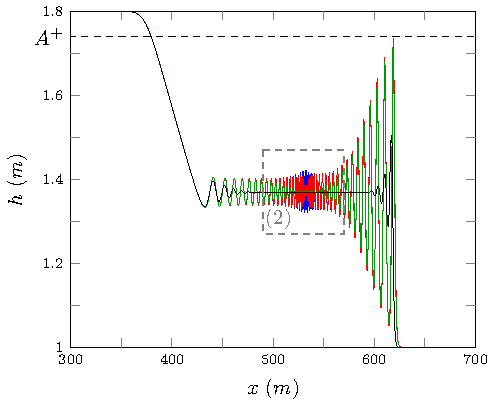
\includegraphics[width=0.7\textwidth]{pics/results/SDB/numsols/alpha10/1-figure0.pdf}
\end{subfigure}
\begin{subfigure}{\textwidth}
	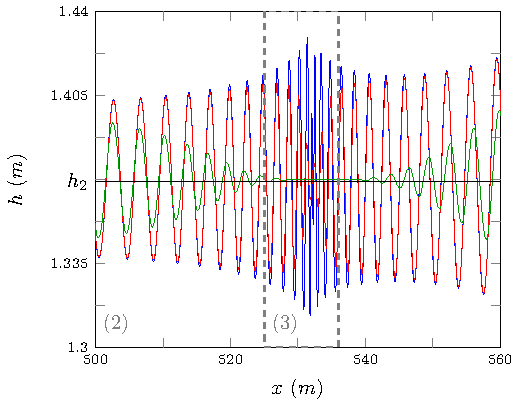
\includegraphics[width=0.5\textwidth]{pics/results/SDB/numsols/alpha10/2-figure0.pdf}
	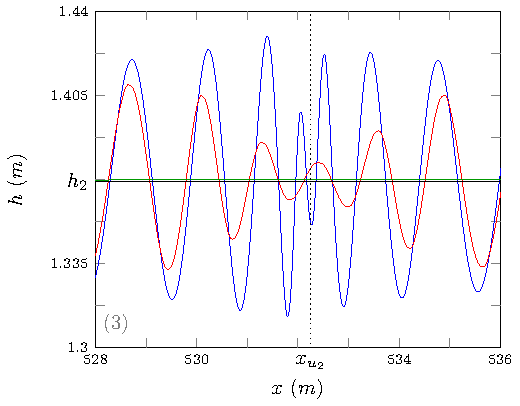
\includegraphics[width=0.5\textwidth]{pics/results/SDB/numsols/alpha10/3-figure0.pdf}
\end{subfigure}
\caption{Numerical results of $\mathcal{V}_3$  at $t= 30s$ for the smooth dam-break problem with $\alpha = 0.1m$ for $\Delta x = 10/2^{10}m$ ({\color{blue} \solidrule}), $10/2^8m$ ({\color{red} \solidrule}), $10/2^6m$ ({\color{green!60!black} \solidrule}) and $10/2^{4}m$ ({\color{black} \solidrule}).}
\label{fig:o3a20dxlimcdexp}
\end{figure}

%smoothing for El as well
%add S_2
Since this our numerical results have poorer convergence and conservation and cannot be found in the literature, we resort to using many different methods to support the numerical solutions of $\mathcal{V}_3$. To remove the possibility that some effect from the refomulation of the Serre equations or the elliptic solver of the $\mathcal{V}_i$ methods are the cause we use make use of $\mathcal{G}$ and $\mathcal{E}$. $\mathcal{G}$, $\mathcal{E}$, $\mathcal{V}_1$ and $\mathcal{V}_3$ are applied to the same initial conditions with the same grid resolutions as above and the results were plotted in Figure \ref{fig:MODlim}. $\mathcal{V}_2$ has been omitted from this figure for clarity because its solution is very close to $\mathcal{V}_3$. 

The first observation is that $\mathcal{V}_1$ has not recovered a growth behaviour. This is because $\mathcal{V}_1$ is very diffusive \cite{Zoppou-etal-2017}, dampening these oscillations. To resolve such behaviour for $\mathcal{V}_1$ would require restrictively small $\Delta x$ and as such this has not been observed in the simulations. Secondly, all high-order methods recover this growth behaviour and disagree only in the region around $x_{u_2}$. The absence of the growth behaviour in the findings of \citet{El-etal-2006} is the result of smoothing of the initial conditions \cite{El-Hoefer-2016-11}.

Generally dispersive methods overestimate the size and number of oscillations of the true solution while diffusive methods underestimate the size and number of oscillations in the true solution. Since $\mathcal{V}_3$ is diffusive as can be seen in Figure \ref{fig:o3a20dxlimcdexp} and $\mathcal{G}$ is dispersive the true analytic solution should exist between $\mathcal{V}_3$ and $\mathcal{G}$. As $\mathcal{G}$ and $\mathcal{V}_3$ have the same number of oscillations we expect that the true solution will have the same number of oscillations with different amplitudes. $\mathcal{G}$ has very similar numerical solutions to $\mathcal{V}_2$ and $\mathcal{V}_3$  which are preferred by the authors due to their robustness and superior conservation of quantities. 

\begin{figure}
\centering
\begin{subfigure}{\textwidth}
	\centering
	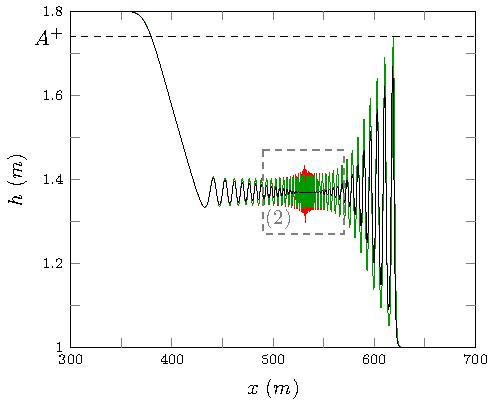
\includegraphics[width=0.7\textwidth]{pics/results/SDB/numsols/modelcomppalpha10dx10/1-figure0.pdf}
\end{subfigure}
\begin{subfigure}{\textwidth}
	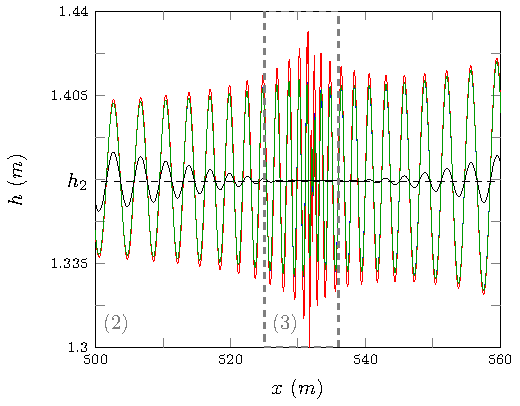
\includegraphics[width=0.5\textwidth]{pics/results/SDB/numsols/modelcomppalpha10dx10/2-figure0.pdf}
	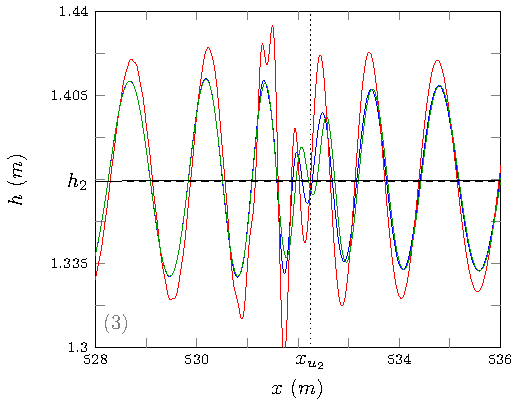
\includegraphics[width=0.5\textwidth]{pics/results/SDB/numsols/modelcomppalpha10dx10/4-figure0.pdf}
\end{subfigure}
\caption{Numerical results for the smooth dam-break problem with $\alpha = 0.1m$ and $\Delta x = 10/2^{10}m$
for $\mathcal{G}$ ({\color{blue} \solidrule}), $\mathcal{E}$ ({\color{red} \solidrule}), $\mathcal{V}_3$ ({\color{green!60!black} \solidrule}) and $\mathcal{V}_1$ ({\color{black} \solidrule}).}
\label{fig:MODlim}
\end{figure}

These results demonstrate that while our numerical results have not converged as $\Delta x \rightarrow 0$ the agreement of all the discussed methods of sufficiently high order indicates that these results are representative of actual solutions of the smoothed dam-break problem with low $\alpha$ for the Serre equations. This is the same behaviour that we observe for $\mathcal{V}_2$ and $\mathcal{V}_3$ with the same $\Delta x$ and $\Delta t$ for the dam-break.


%--------------------------------------------------------------------------------
\subsection{Long time}\label{subsubsec:LT}
%--------------------------------------------------------------------------------
To assess long term behaviour a smoothed dam-break was solved by $\mathcal{V}_3$ with the same parameters on a larger domain $x \in [-900m, 1800m]$ for a longer time $t \in [0,300s]$. The results of $\mathcal{V}_3$ with $\alpha = 0.1m$ and $\Delta x = 10/2^{9}m$ and $10/2^{8}m$ at $t = 300s$ are presented in Figure \ref{fig:FVcomplonga20}. For this problem these parameters result in the growth behaviour, however after sufficient time this growth behaviour has decayed back into a flat behaviour although there are still small oscillations present in the middle region. 

To track the decaying of the oscillations for $\mathcal{V}_3$'s solution around $x_{u_2}$ a snapshot of the area around $x_{u_2}$ has been plotted for different times in Figure \ref{fig:FVlongcemt500}. It can be seen that at $t =30s$ the solution exhibits the growth behaviour but as time progresses the region around $x_{u_2}$ has decayed into the node behaviour by $t=100s$ and then into the flat behaviour observed at $t=200s$ and $t=300s$. This is most likely due to the accumulation of diffusive errors of the numerical method with Figure \ref{fig:FVcomplonga20} demonstrating that over this time span we are not close to convergence of the numerical results.   

%coarsefinecomparison
\begin{figure}
	\centering
	\begin{subfigure}{\textwidth}
		\centering
		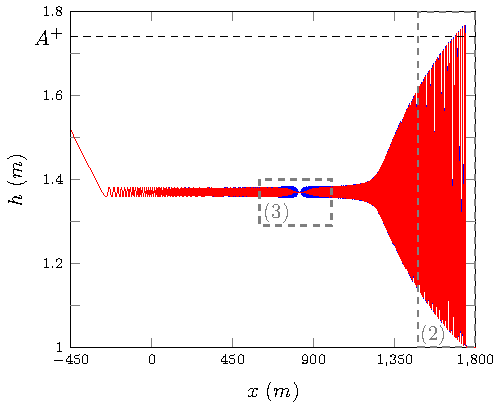
\includegraphics[width=0.7\textwidth]{pics/results/SDB/numsols/300s/CF0t300s.pdf}
	\end{subfigure}
	\begin{subfigure}{\textwidth}
		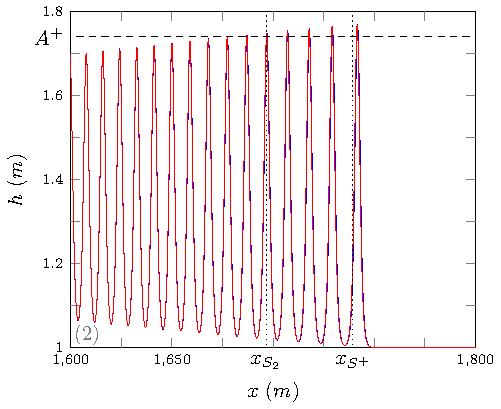
\includegraphics[width=0.5\textwidth]{pics/results/SDB/numsols/300s/CF1t300s.pdf}
		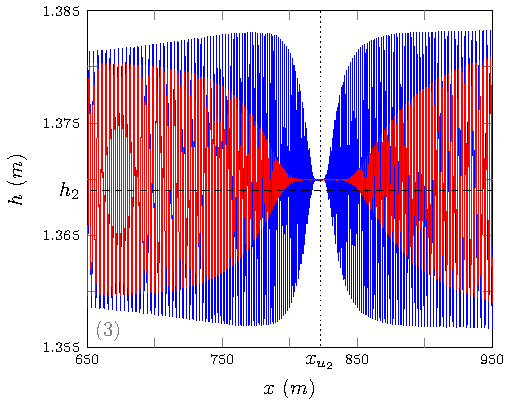
\includegraphics[width=0.5\textwidth]{pics/results/SDB/numsols/300s/CF2t300s.pdf}
	\end{subfigure}
	\caption{Numerical solution of smooth dam-break problem at $t=300s$ by $\mathcal{V}_3$ with $\alpha = 0.1m$ for $\Delta x = 10/2^{9}m$ ({\color{blue} \solidrule}) and $10/2^{8}m$ ({\color{red} \solidrule}).}
	\label{fig:FVcomplonga20}
\end{figure}

\begin{figure}
\centering
\begin{subfigure}{0.5\textwidth}
	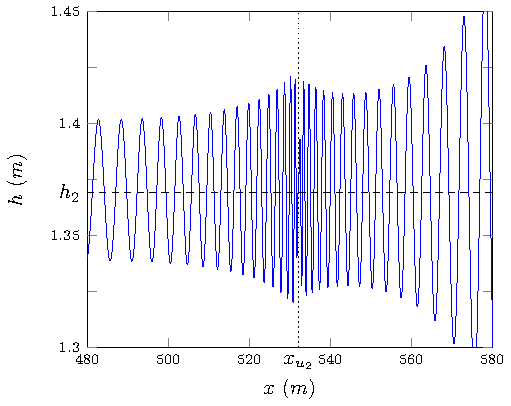
\includegraphics[width=\textwidth]{pics/results/SDB/numsols/300s/evolve30s.pdf}
	\subcaption*{\hspace{10 mm}$t=30s$}
\end{subfigure}%
\begin{subfigure}{0.5\textwidth}
	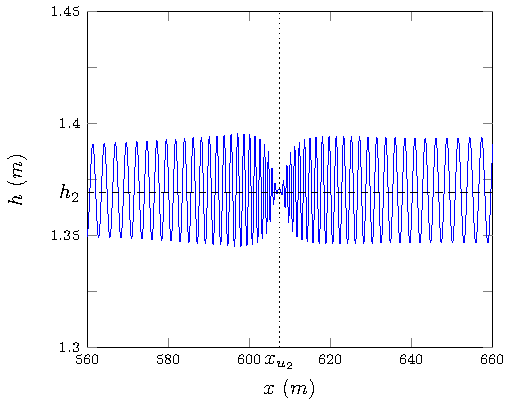
\includegraphics[width=\textwidth]{pics/results/SDB/numsols/300s/evolve100s.pdf}
	\subcaption*{\hspace{10 mm} $t=100s$}
\end{subfigure}
\begin{subfigure}{0.5\textwidth}
	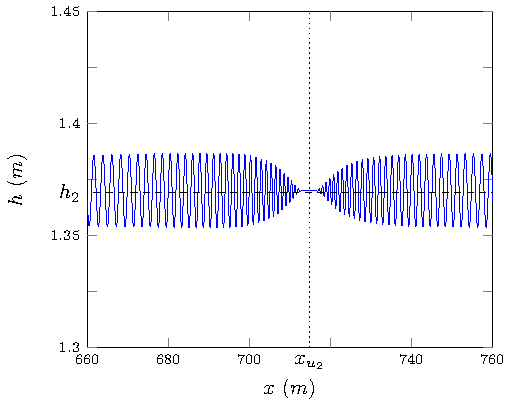
\includegraphics[width=\textwidth]{pics/results/SDB/numsols/300s/evolve200s.pdf}
	\subcaption*{\hspace{10 mm}$t=200s$}
\end{subfigure}%
\begin{subfigure}{0.5\textwidth}
	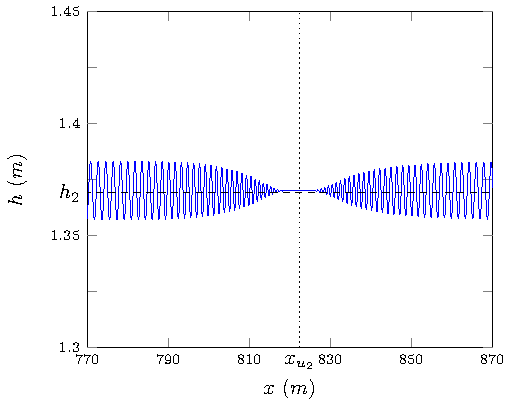
\includegraphics[width=\textwidth]{pics/results/SDB/numsols/300s/evolve300s.pdf}
	\subcaption*{\hspace{10 mm}$t=300s$}
\end{subfigure}

\caption{Numerical solution of the smooth dam-break problem by $\mathcal{V}_3$ with $\alpha = 0.1m$ and $\Delta x = 10/2^{9}m$ at various times.}
\label{fig:FVlongcemt500}
\end{figure}


\subsection{Shallow water wave equation comparison}
The shallow water wave equations have been used as a guide for the mean behaviour of the solution of the Serre equations for the dam-break problem in the literature \cite{Hank-etal-2010-2034,Mitsotakis-etal-2014}. We assess their applicability by plotting $h - h_2$ and $u - u_2$ for the smoothed dam-break problem with $\alpha = 0.1m$ and $\Delta x = {10}/{2^9}m$ in Figure \ref{fig:UHSWWcomp30sall} for $t= 30s$ and Figure \ref{fig:UHSWWcomp300sall} for $t= 300s$. 

From these results it can be seen that over short time spans both $h_2$ and $u_2$ are good approximations to the mean behaviour of the fluid with both plots oscillating around $0$. However after sufficient time the mean velocity and height of the bore have diverged slightly from the shallow water wave equation values $h_2$ and $u_2$. With $h_2$ being an underestimate and $u_2$ being an overestimate. While Figure \ref{fig:FVcomplonga20} demonstrates that $S_2$ is a worse approximation than $h_2$ and $u_2$.

\begin{figure}
	\centering
	\begin{subfigure}{\textwidth}
		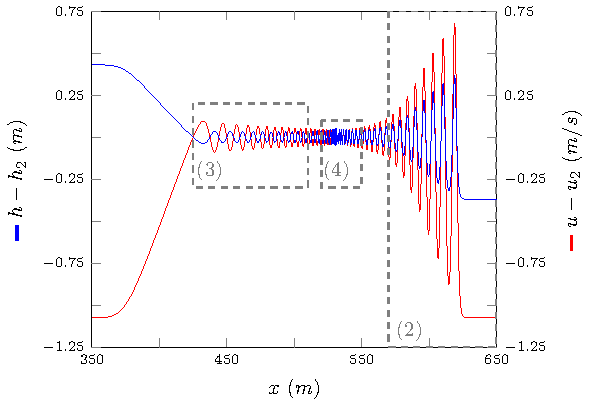
\includegraphics[width=0.5\textwidth]{pics/results/SDB/numsols/SWWCOMP/30s/0.pdf}
		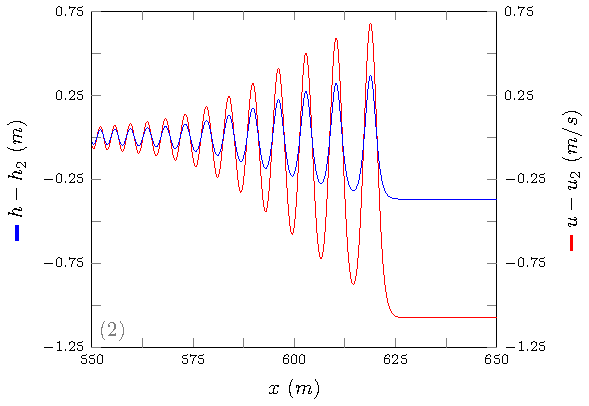
\includegraphics[width=0.5\textwidth]{pics/results/SDB/numsols/SWWCOMP/30s/2.pdf}
	\end{subfigure}
	\begin{subfigure}{\textwidth}
		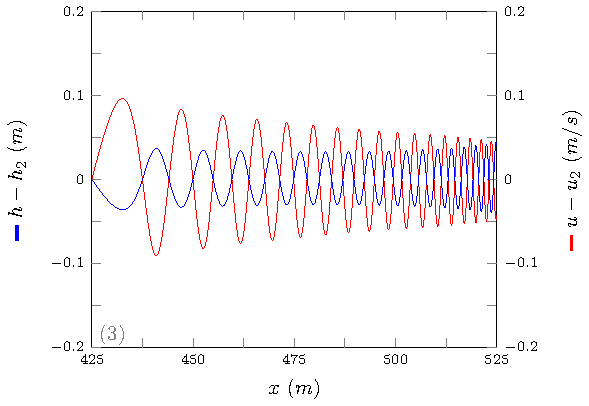
\includegraphics[width=0.5\textwidth]{pics/results/SDB/numsols/SWWCOMP/30s/1.pdf}
		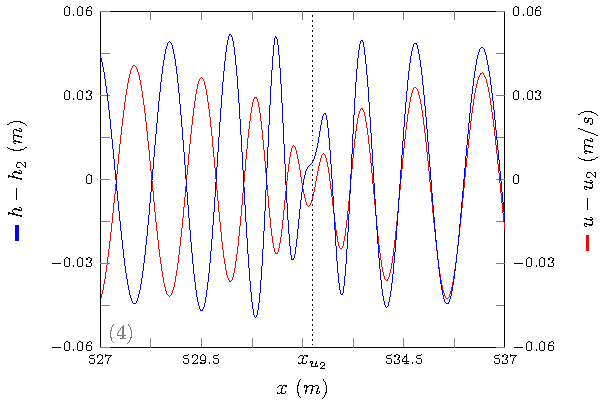
\includegraphics[width=0.5\textwidth]{pics/results/SDB/numsols/SWWCOMP/30s/3.pdf}
	\end{subfigure}
	\caption{$h - h_2$ ({\color{blue} \solidrule}) and $u - u_2$ ({\color{red} \solidrule}) for numerical solution of the smooth dam-break by $\mathcal{V}_3$ with $\alpha = 0.1m$ and $\Delta x = 10/2^{9}m$ at $t=30s$ as in Figure \ref{fig:o3a20dxlimcdexp}.}
	\label{fig:UHSWWcomp30sall}
\end{figure}

\begin{figure}
	\centering
\begin{subfigure}{\textwidth}
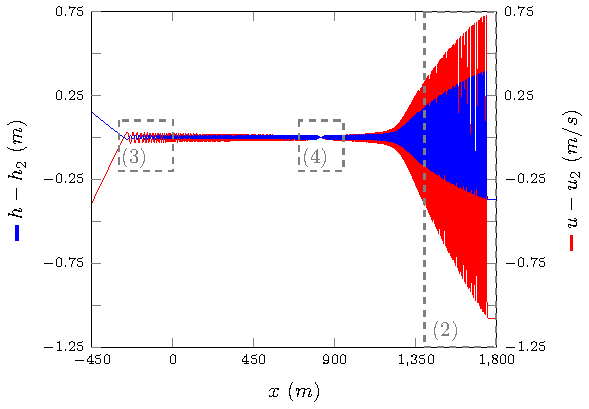
\includegraphics[width=0.5\textwidth]{pics/results/SDB/numsols/SWWCOMP/300s/0.pdf}
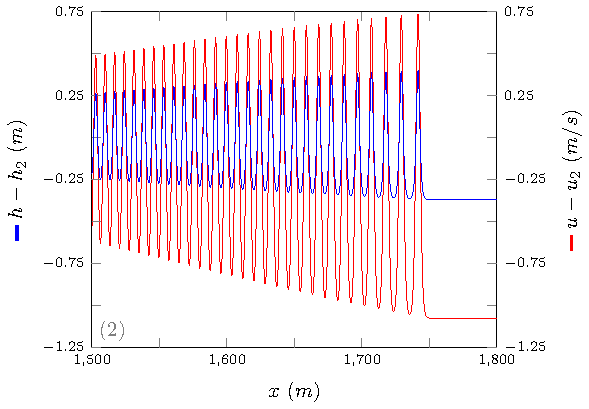
\includegraphics[width=0.5\textwidth]{pics/results/SDB/numsols/SWWCOMP/300s/2.pdf}
\end{subfigure}
\begin{subfigure}{\textwidth}
	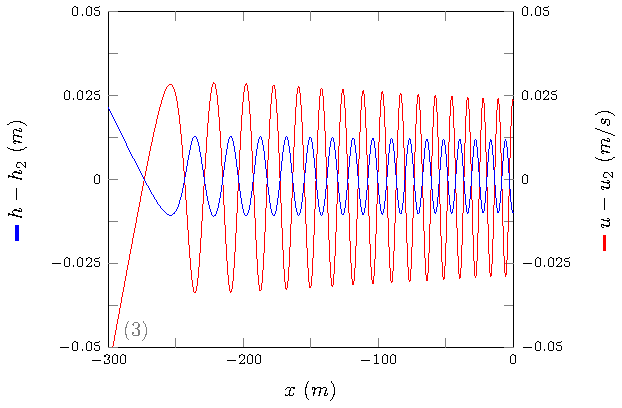
\includegraphics[width=0.5\textwidth]{pics/results/SDB/numsols/SWWCOMP/300s/1.pdf}
	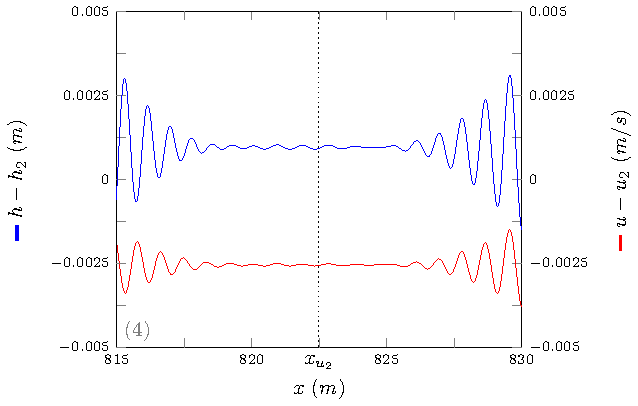
\includegraphics[width=0.5\textwidth]{pics/results/SDB/numsols/SWWCOMP/300s/3.pdf}
\end{subfigure}
	\caption{$h - h_2$ ({\color{blue} \solidrule}) and $u - u_2$ ({\color{red} \solidrule}) for numerical solution of the smooth dam-break by  $\mathcal{V}_3$ with $\alpha = 0.1m$ and $\Delta x = 10/2^{9}m$ at $t=300s$ as in Figure \ref{fig:FVcomplonga20}.}
	\label{fig:UHSWWcomp300sall}
\end{figure}

\subsubsection{Contact discontinuity}
The contact discontinuity is the location of the node in the node behaviour \cite{El-etal-2006} and the growth of the oscillations in the growth behavior, we have demonstrated that this is at about $x_{u_2}$ as can be seen in Figures \ref{fig:o3a9dxlimcdexp} and \ref{fig:o3a20dxlimcdexp}. Figures \ref{fig:UHSWWcomp30sall} and \ref{fig:UHSWWcomp300sall} show a more fundamental property of the contact discontinuity, that it is the transition between when $h$ and $u$ are anti-phase to the left and when $h$ and $u$ are in-phase to the right.

By inspecting the phase velocity for the linearised Serre equations
\begin{linenomath*}
		\begin{gather}
		\upsilon_p = u \pm \sqrt{gh} \sqrt{\frac{3}{h^2 k^2 + 3}}
		\end{gather}
\end{linenomath*}
with wave number $k$, it can be seen that as $k \rightarrow \infty$ then $\upsilon_p \rightarrow u$ and as $k \rightarrow 0$ then $\upsilon_p \rightarrow u \pm \sqrt{gh}$. Therefore when $u$ and $h$ are anti-phase this corresponds to the negative branch of the phase velocity $u - \sqrt{gh} \sqrt{{3}/\left({h^2 k^2 + 3}\right)}$ and when $u$ and $h$ are in-phase this corresponds to the positive branch  $u + \sqrt{gh} \sqrt{{3}/\left({h^2 k^2 + 3}\right)}$. So that the contact discontinuity is the location of the highest wave numbers and it travels at speed $u$ which would be the mean velocity inside the bore. This explains why the behaviour around the contact discontinuity is sensitive to smoothing of the initial conditions and diffusivity of the method.

A range of different mean bore speeds where modelled with smoothed dam-break problems by fixing $h_0=1m$ and varying $h_1$ to allow for different aspect ratios and thus different bore speeds. The results are plotted in Figure \ref{fig:CDspeed} fwhich shows that the contact discontinuity travels at a speed close to $u_2$ for a range of mean bore speeds. 

These results demonstrate that while $h_2$ and $u_2$ are not exactly the mean behaviour of the bore for the Serre equations the two are highly correlated across a range of different smoothed dam-break problems and so the analytic solutions of the shallow water wave equations are a good guide for the mean behaviour of the Serre equations.
\begin{figure}
	\centering
	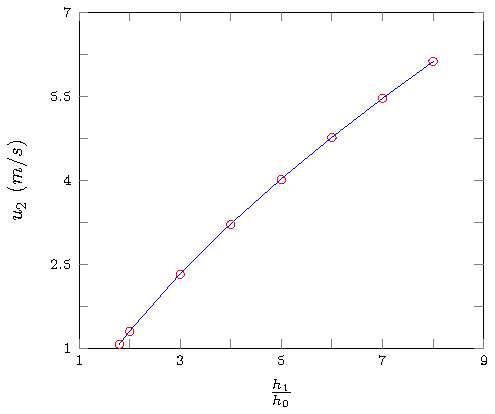
\includegraphics[width=0.5\textwidth]{pics/results/SDB/CDspeed/speed.pdf}
	\caption{$u_2$ ({\color{blue} \solidrule}) and speed of the contact discontinuity ({\color{red} $\circ$})  for numerical solutions of smoothed dam-break problems with different aspect ratios ($h_1 /h_0$) by $\mathcal{V}_3$ where $\alpha = 0.1m$ and $\Delta x = 10/2^{9}m$ at $t=100s$.}
	\label{fig:CDspeed}
\end{figure}


%%% a plus 
\subsection{Whitham modulation comparison}
The expressions for the leading wave amplitude $A^+$ and speed $S^+$ obtained by \cite{El-etal-2006} are asymptotic results and so we are interested in how our numerical results behave over time. Thus for the dam-break problem in Figure \ref{fig:FVcomplonga20} the peak amplitude in region IV ($A$) was plotted over time in Figure \ref{fig:FVlonga20aplus}. It can seen that $A$ approaches a value larger than $A^+$ over time. We find that as $\alpha \rightarrow 0$ and $\Delta x \rightarrow 0$ $A$ converges away from $A^+$ in this time scale for this aspect ratio. Thus it appears that the true solution of the dam-break for the Serre equations has an amplitude in region IV slighlty above $A^+$. This is not inconsistent with the results of \cite{El-etal-2006} as their scale comparing $A^+$ to $A$ is too large to see such a small difference. From Figure \ref{fig:FVcomplonga20} it can be seen that while $S^+$ does not precisely predict the bore speed it is a better prediction than $S_2$.

These results together with those of \citet{El-etal-2006} demonstrate that $A$ and $A^+$ are highly correlated across a range of different smoothed dam-break problems, but for a given problem these two are not precisely equal for our numerical results.
\begin{figure}
	\centering
    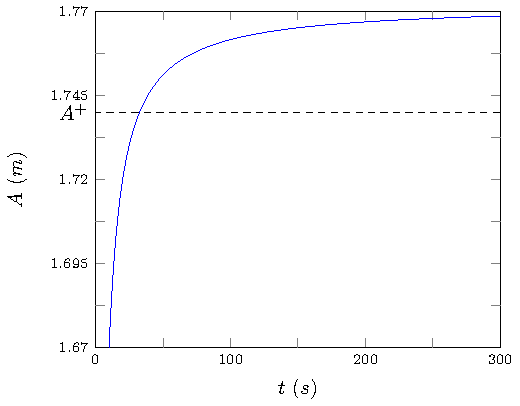
\includegraphics[width=0.5\textwidth]{pics/results/SDB/numsols/300s/a.pdf}
	\caption{Leading wave height plotted over time for the numerical solution of the smooth dam-break problem by $\mathcal{V}_3$ with $\alpha = 0.1m$ for $\Delta x = 10/2^{9}m$ ({\color{blue} \solidrule}) as in Figure \ref{fig:FVcomplonga20}.}
	\label{fig:FVlonga20aplus}
\end{figure}

%energy break down
\subsection{Energy Breakdown}
The Hamiltonian \eqref{eqn:Hamildef} has $3$ terms representing in order, horizontal kinetic energy $hu^2$, vertical kinetic energy $\frac{h^3}{3}\frac{\partial u}{\partial x}$ and gravitational potential energy $gh^2$. It might be expected that the oscillations of the undular bore such as in Figure \ref{fig:FVcomplonga20} would result in significant vertical energies. However, Figure \ref{fig:PHTa12all} demonstrates that this is not the case, as the total vertical kinetic energy in the system is insignificant relative to the other energies. This plot also demonstrates that even with dispersive terms and large oscillations the drivers of change in the dam-break problem are the transfer of gravitational potential energy into horizontal kinetic energy which occurs slowly.

\begin{figure}
	\centering
	\begin{subfigure}{\textwidth}
		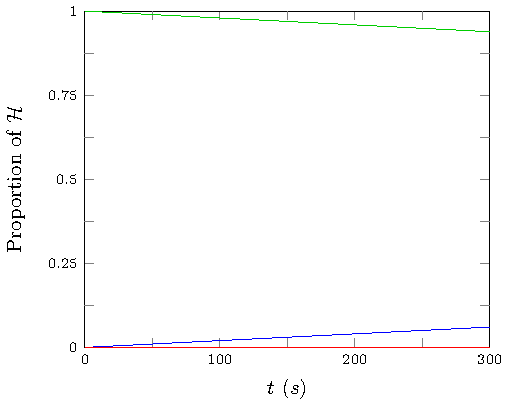
\includegraphics[width=0.5\textwidth]{pics/results/SDB/H/Time/HFT-figure0.pdf}
		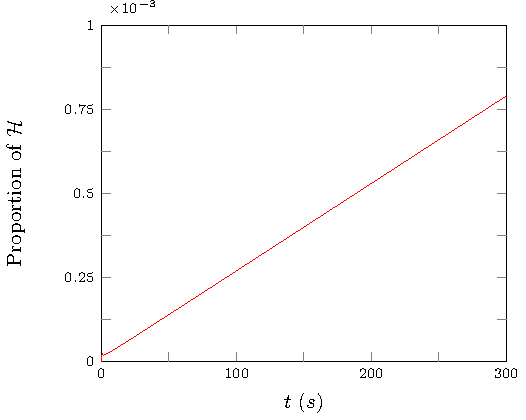
\includegraphics[width=0.5195\textwidth]{pics/results/SDB/H/Time/TT-figure0.pdf}
	\end{subfigure}
	\caption{Proportion of $\mathcal{H}$ made up by horizontal kinetic energy ({\color{blue} \solidrule}), vertical kinetic energy ({\color{red} \solidrule}) and gravitational potential energy ({\color{green!80!black} \solidrule}) for $\mathcal{V}_3$'s solution of the smooth dam-break problem with $\alpha = 0.1m$ and $\Delta x = 10/2^{9}m$ over time as in Figure \ref{fig:FVcomplonga20}.}
	\label{fig:PHTa12all}
\end{figure}
%--------------------------------------------------------------------------------
\section{Conclusions}
\label{section:Conclusions}
%--------------------------------------------------------------------------------
Utilising two finite difference methods of second-order and three finite difference-volume hybrid methods of various orders an investigation into the smoothed dam-break problem with varying steepness was performed. Four different behaviours were uncovered with the general trend being that an increase in steepness increases the size and number of oscillations in the solution. This study explains the different numericals results in literature involving the solution of the Serre equations applied to the smoothed dam-break problem and also uncovers a new result. We find that while the analytic solution of the shallow water wave equations for the dam-break problem is a good guide to the mean behaviour of the Serre equations the speed and height of the bores do not match up precisely. While the Whitham modulation results for the Serre equations give better predictions than the shallow water wave equations analytic solution it was found that they also do not line up with our numerical results precisely. It was demonstrated that the contact discontinuity corresponds to high wave numbers and thus travels at the mean velocity inside the bore. Lastly it was shown that vertical kinetic energy is negligible for the Serre equations applied to the dam-break problem. 

%more research


%--------------------------------------------------------------------------------
\bibliography{DamBreak}
\bibliographystyle{elsarticle-num-names}
%--------------------------------------------------------------------------------


\end{document}
